\subsection{Experimental setup}
Our experimental setup is as follows \cite{versuchsanleitung}:
First we will have a construction such that we can measure the 
the peaks of a given natrium-, mercury and halogenlamp, you 
can see the setup in figure~\ref{fig:const1}.
After having measured the spectra we will continue and append
the iodine-pipe into the setup, see figure~\ref{fig:const2}.
The pipe is 50 cm long and its diameter is 4 cm. Its inner 
vapour pressure is 0.5 Torr. It will be 
inserted between the lamp and the spectroscope, which is on 
the right side. Here we give some details about the iodine:
\begin{tabular}{| l | l |}
    \hline
    atomic mass   & $126.9 u$ \\
    \hline
    melting point & $113.7^{\circ}$ \\
    \hline
    boiling point & $184.3^{\circ}$
\end{tabular}
\begin{wrapfigure}{r}{0.50\textwidth}
  \begin{center}
    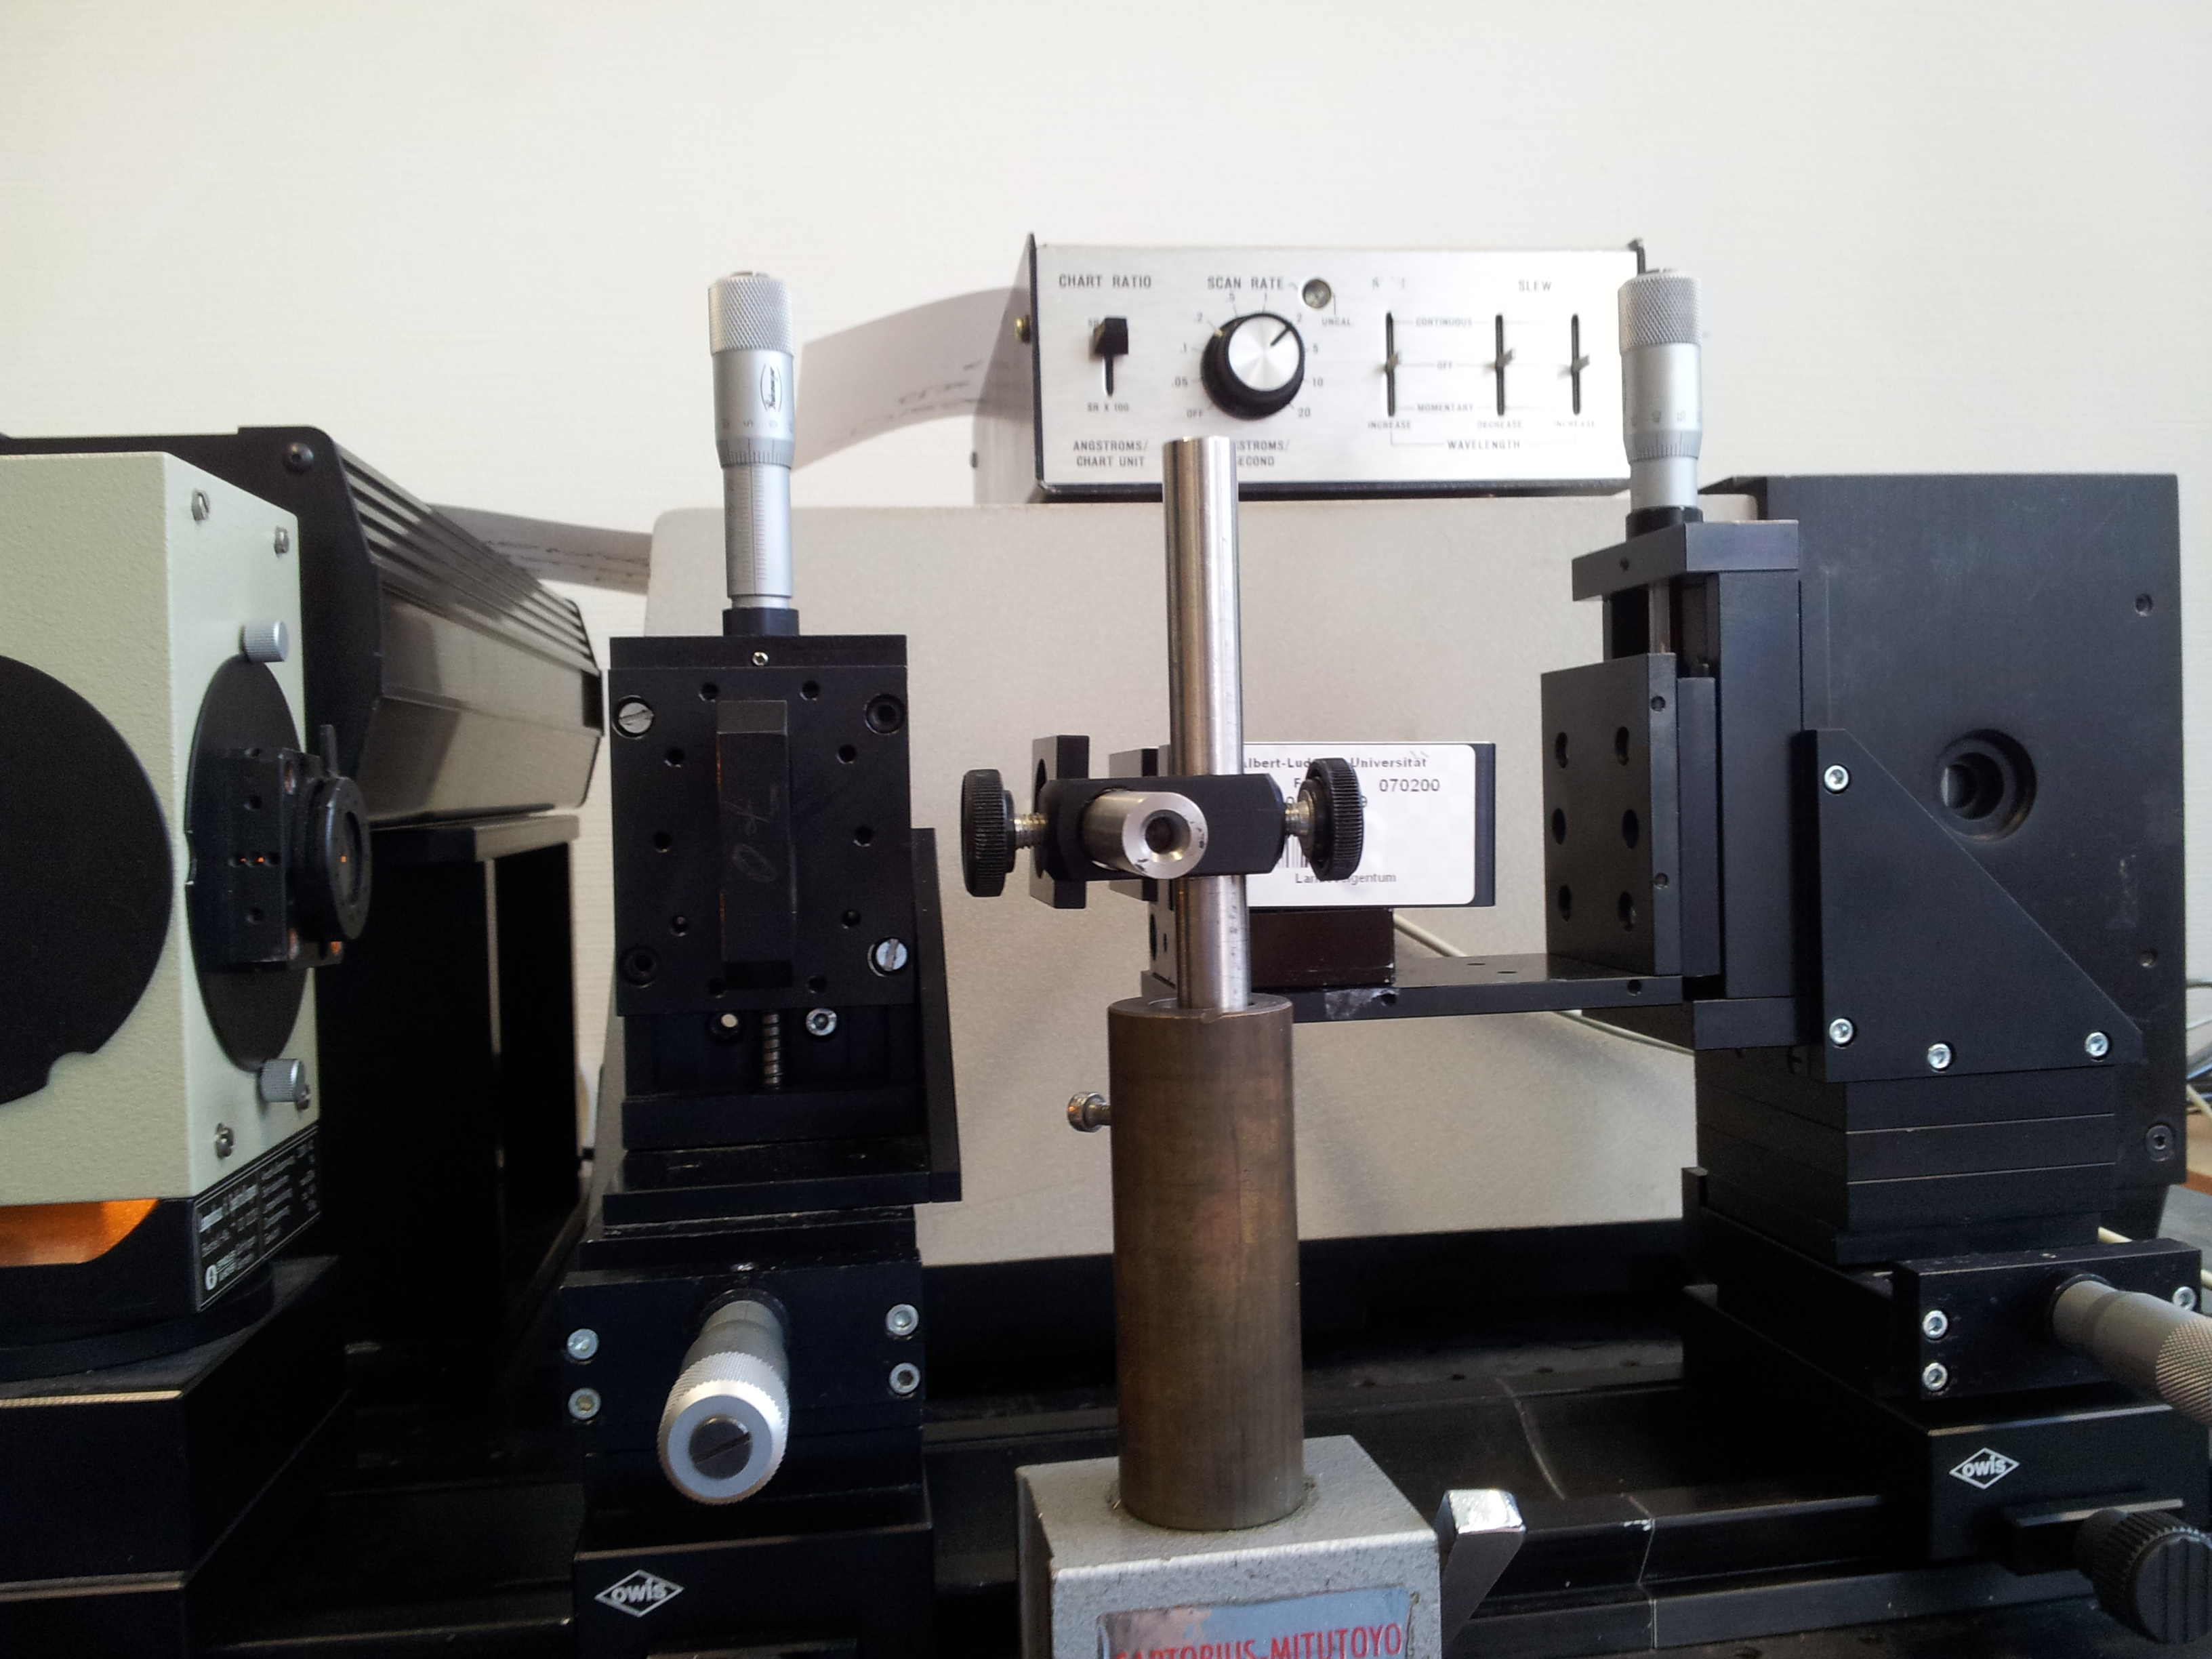
\includegraphics[width=0.47\textwidth]{pics/const1}
  \end{center}
\caption{Photography of the experimental setup when we measure
    the spectra of given lamps.} 
  \vspace{-10pt}
 \label{fig:const1}

\end{wrapfigure}
sample textsample textsample textsample textsample textsample text
sample textsample textsample textsample textsample textsample text
sample textsample textsample textsample textsample textsample text
sample textsample textsample textsample textsample textsample text
sample textsample textsample textsample textsample textsample text
sample textsample textsample textsample textsample textsample text
sample textsample textsample textsample textsample textsample text
sample textsample textsample textsample textsample textsample text
sample textsample textsample textsample textsample textsample text
sample textsample textsample textsample textsample textsample text
sample textsample textsample textsample textsample textsample text
sample textsample textsample textsample textsample textsample text
sample textsample textsample textsample textsample textsample text

\begin{wrapfigure}{l}{0.50\textwidth}
  \begin{center}
    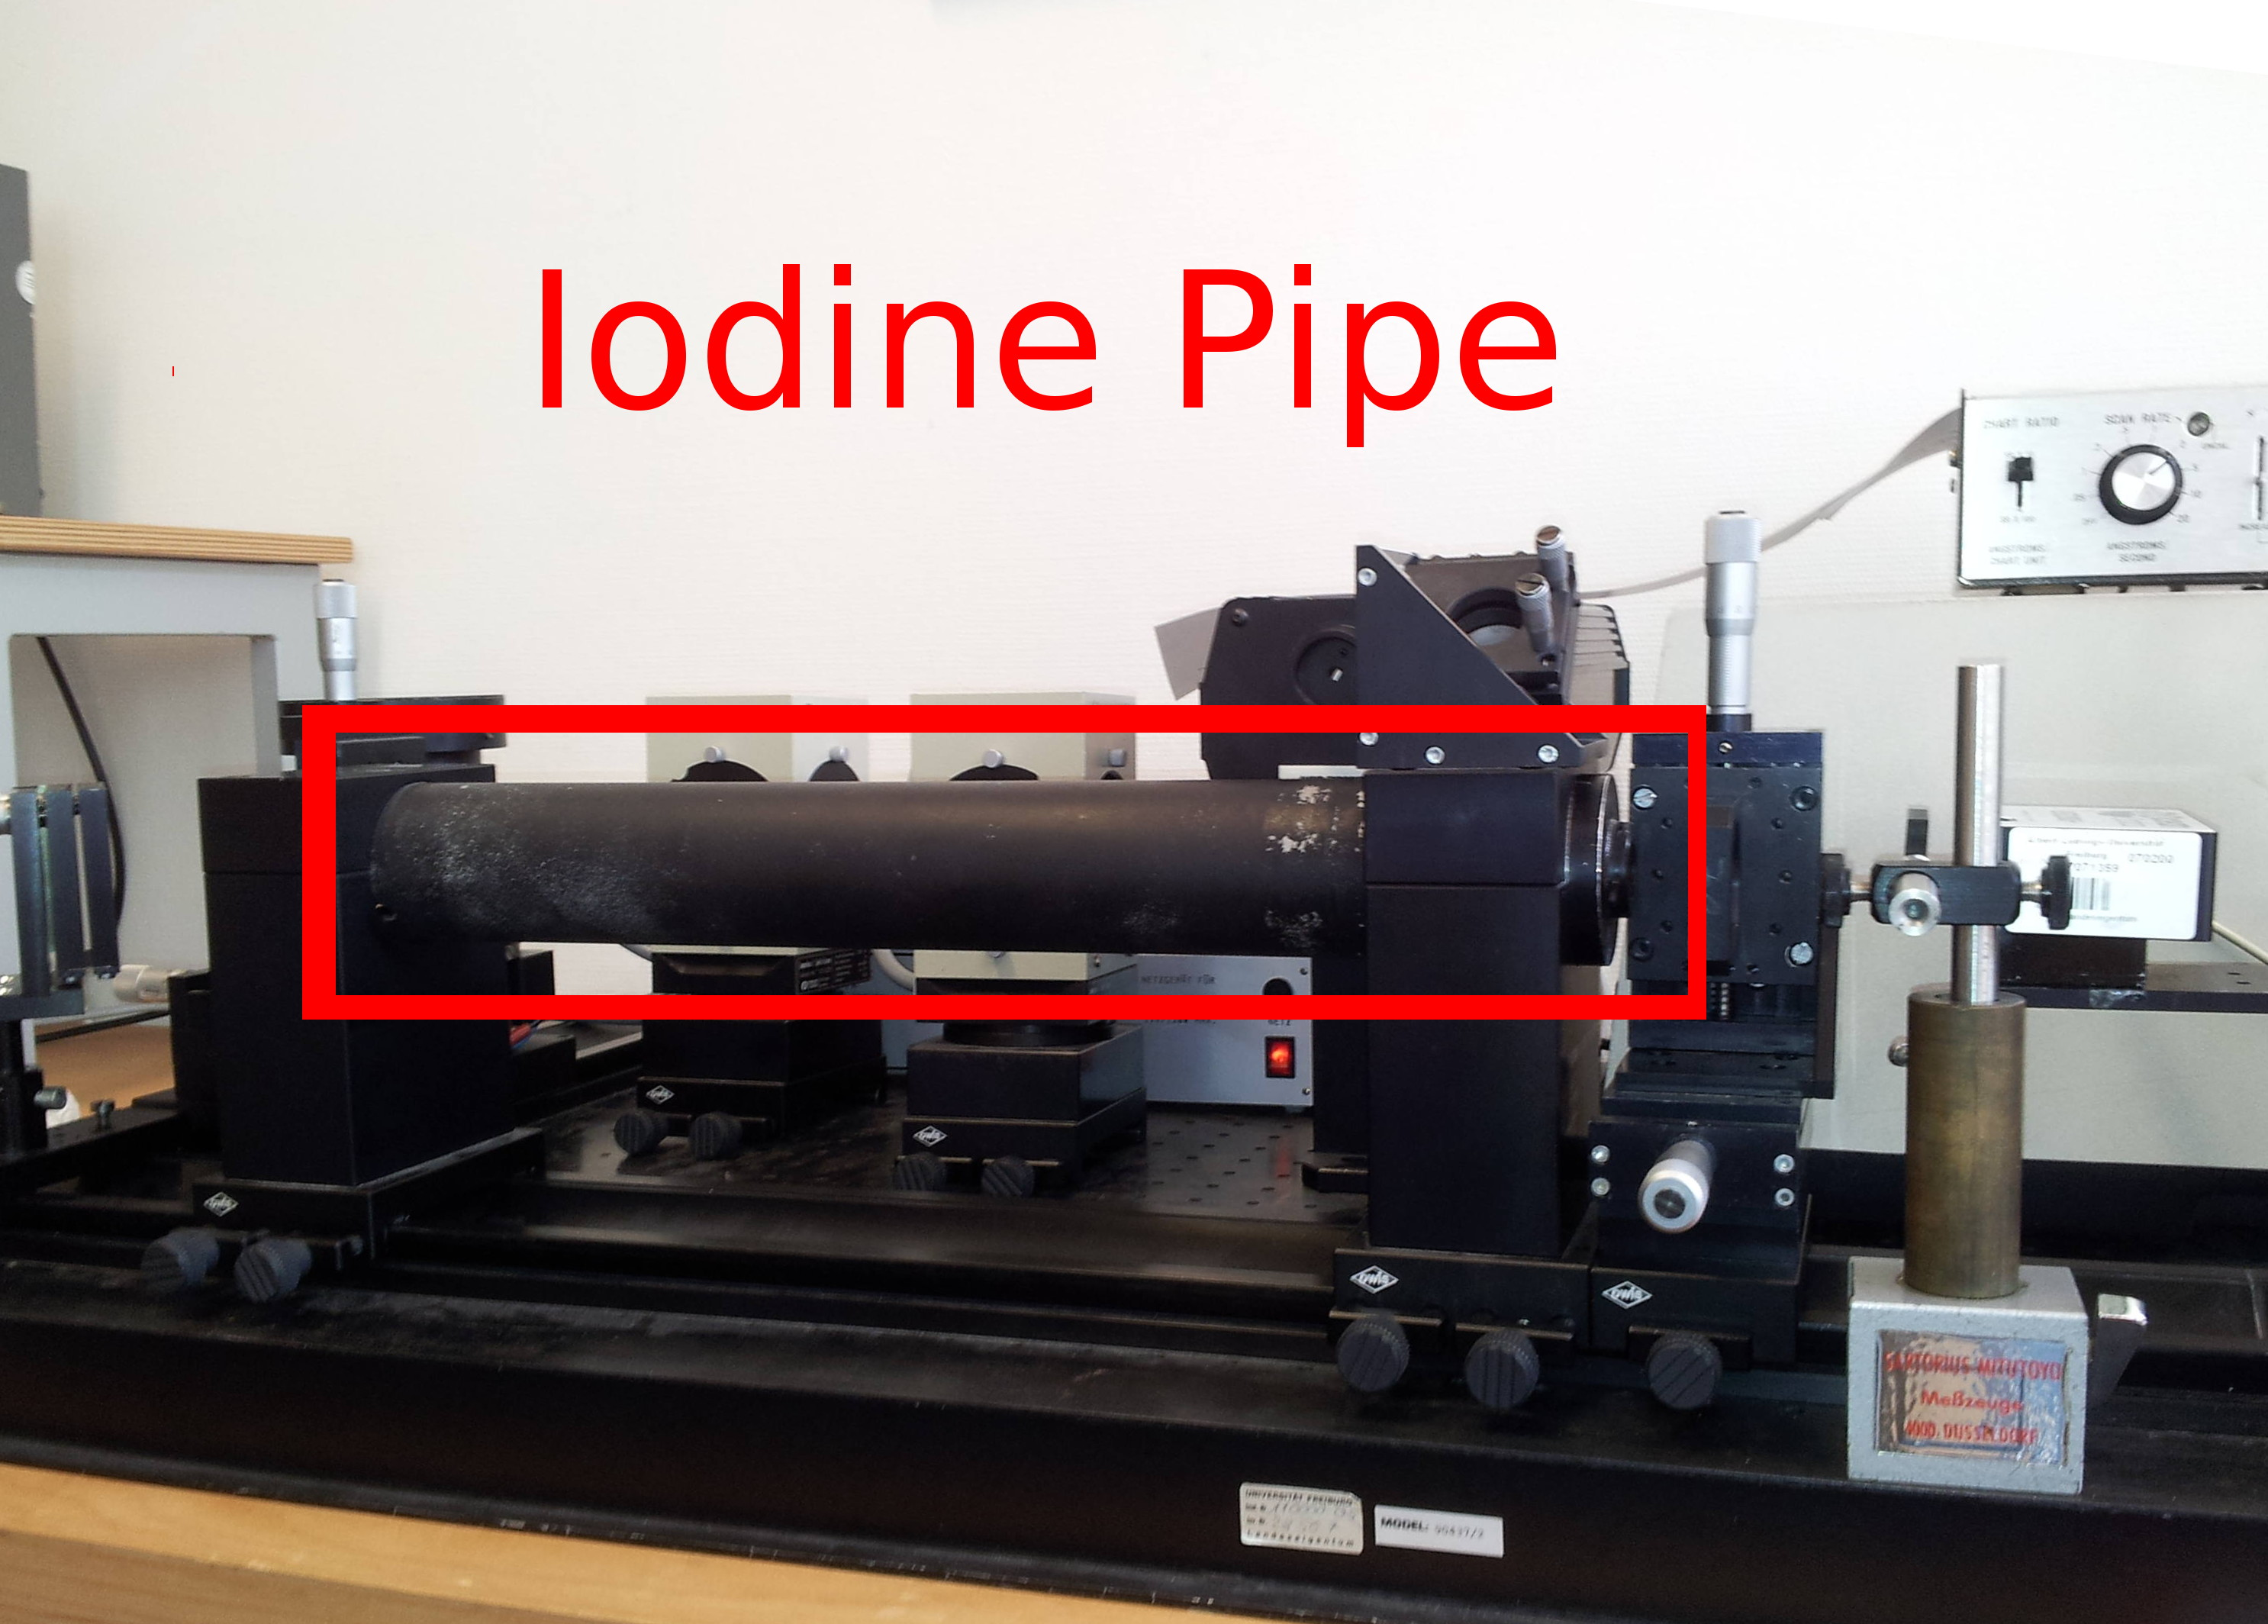
\includegraphics[width=0.47\textwidth]{pics/const2}
  \end{center}
\caption{Photography of the experimental setup with the
    iodinepipe.} 
 \label{fig:const2}

\end{wrapfigure}

sample textsample textsample textsample textsample textsample text
sample textsample textsample textsample textsample textsample text
sample textsample textsample textsample textsample textsample text
sample textsample textsample textsample textsample textsample text
ample textsample textsample textsample textsample textsample text
sample textsample textsample textsample textsample textsample text
sample textsample textsample textsample textsample textsample text
sample textsample textsample textsample textsample textsample text
sample textsample textsample textsample textsample textsample text
sample textsample textsample textsample textsample textsample text
\begin{wrapfigure}{r}{0.50\textwidth}
  \begin{center}
    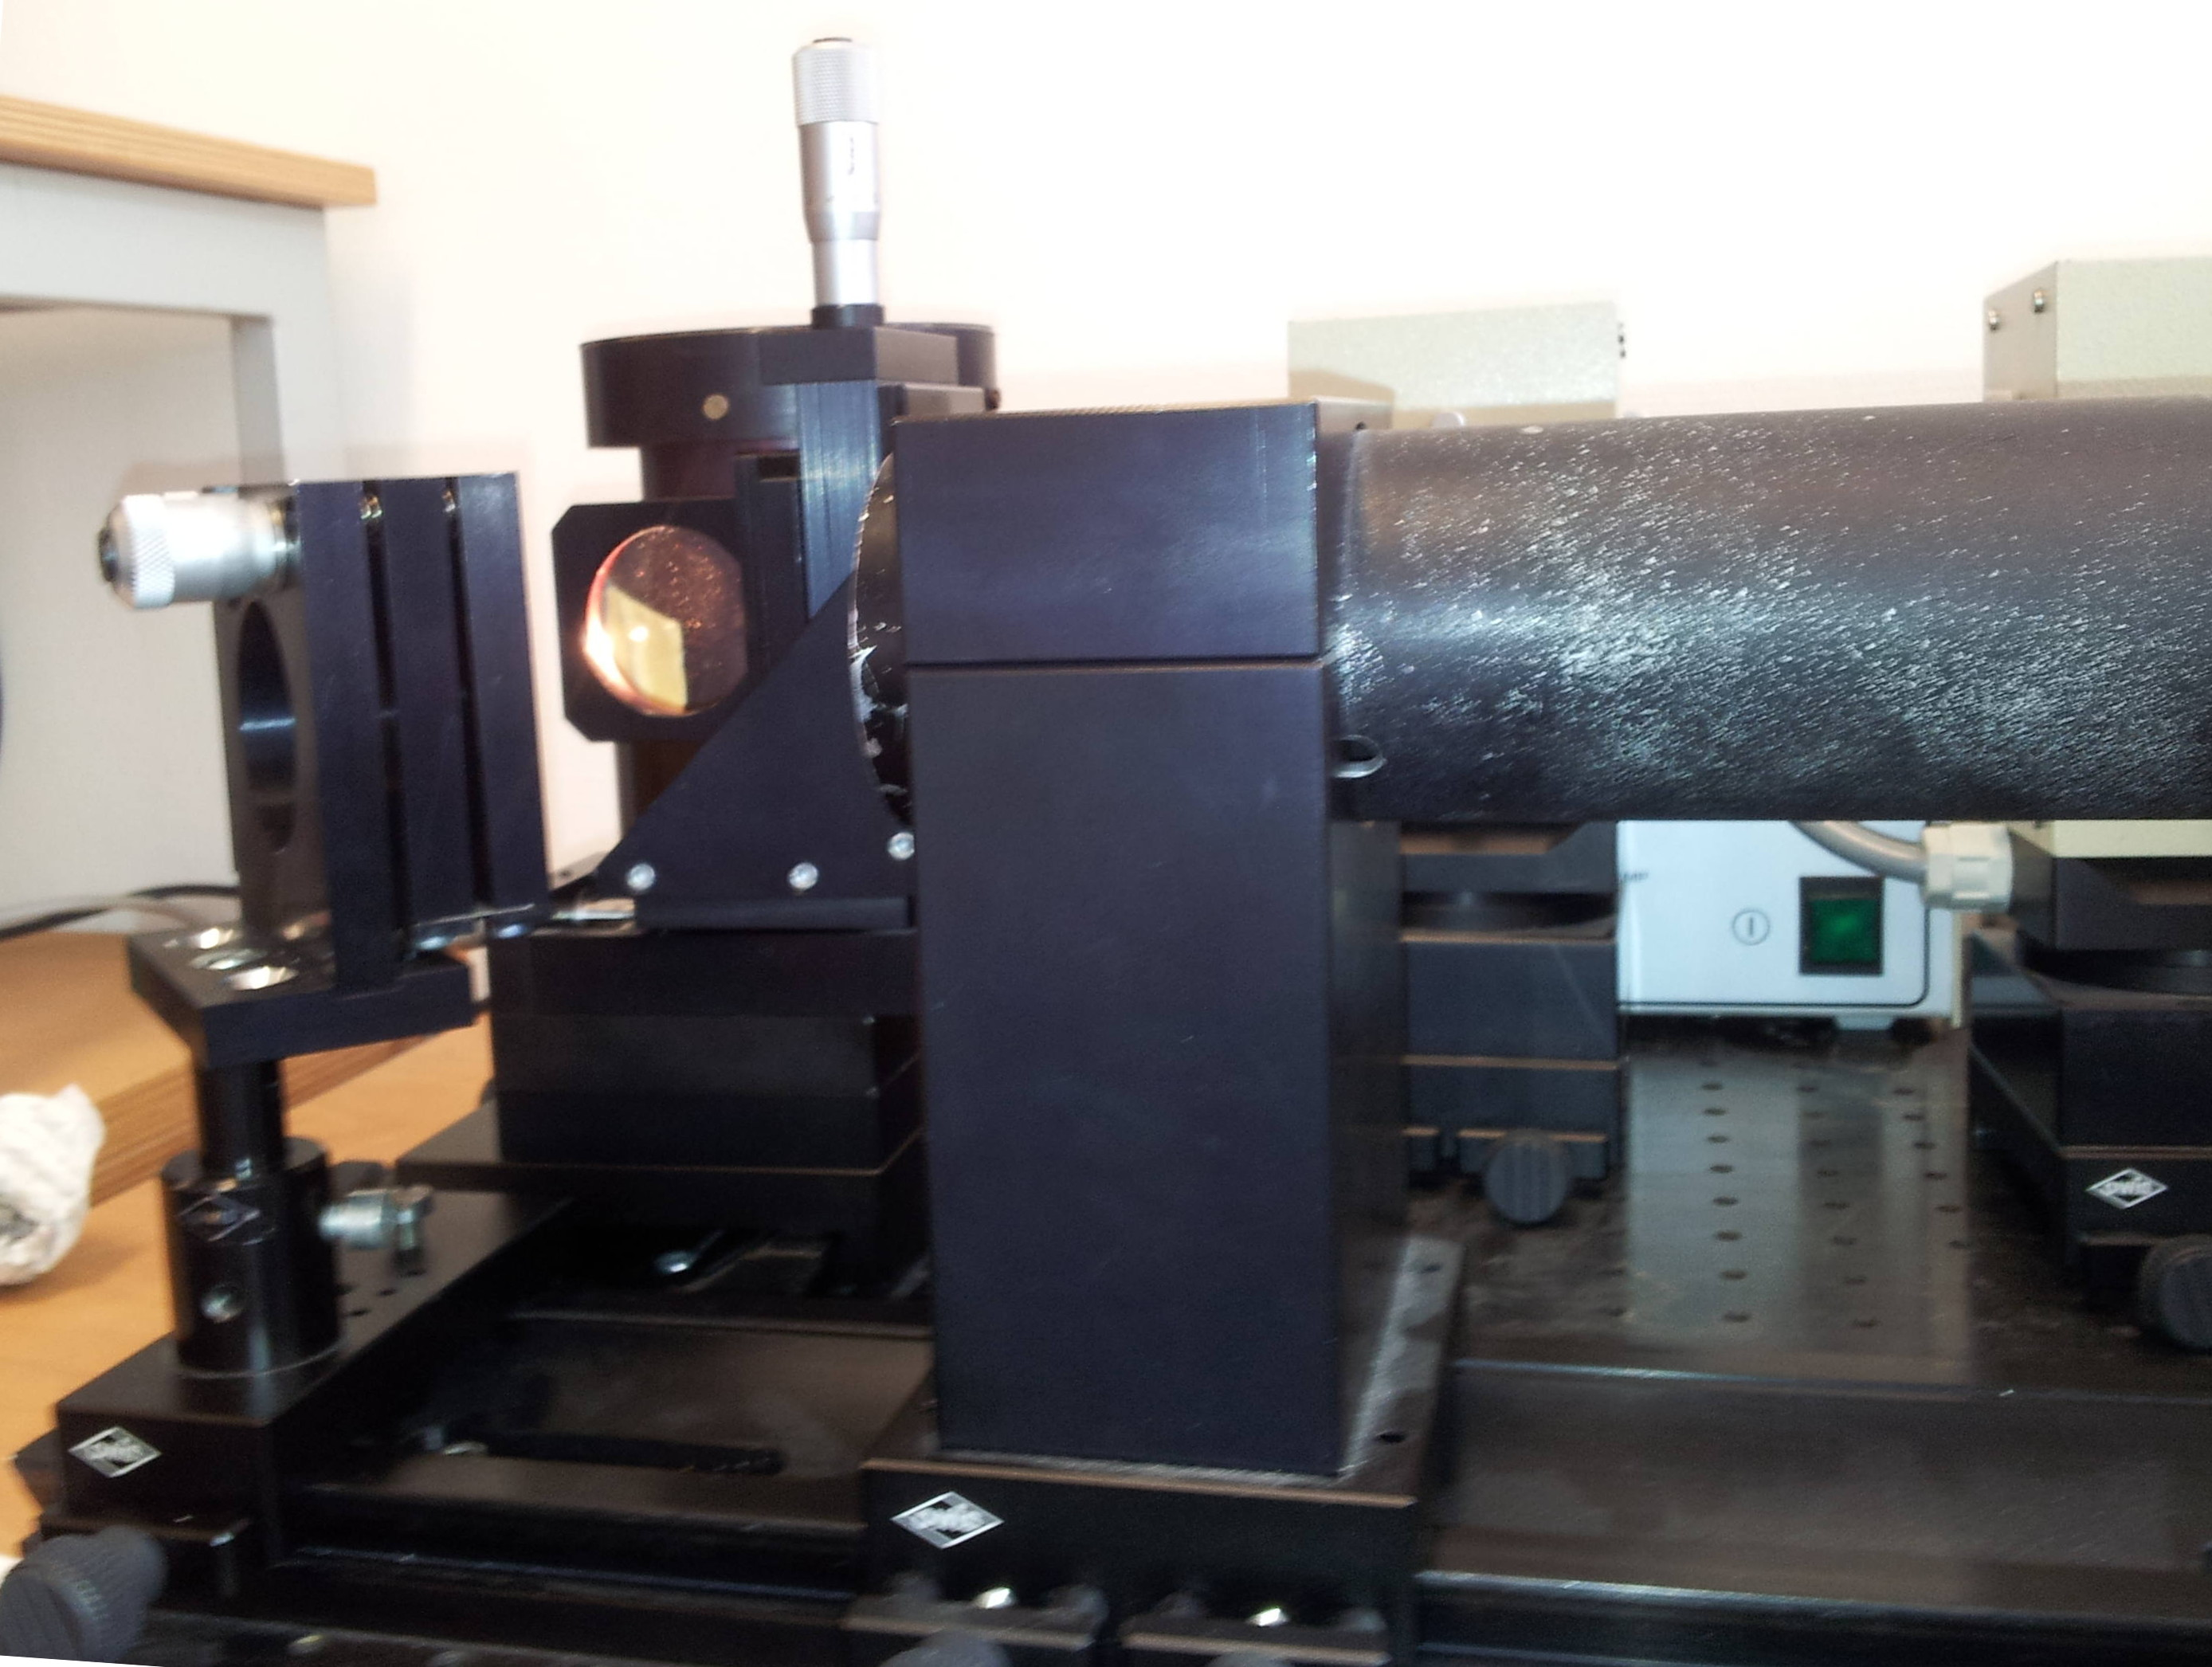
\includegraphics[width=0.47\textwidth]{pics/const4}
  \end{center}
\caption{Photography of the experiment.} 
  \vspace{-10pt}
 \label{fig:const4}

\end{wrapfigure}

sample textsample textsample textsample textsample textsample text
sample textsample textsample textsample textsample textsample text
sample textsample textsample textsample textsample textsample text
sample textsample textsample textsample textsample textsample text
sample textsample textsample textsample textsample textsample text
sample textsample textsample textsample textsample textsample text
\begin{SCfigure} 
\caption{On this photography you can recognize very 
    clearly the spectroscope!!} 
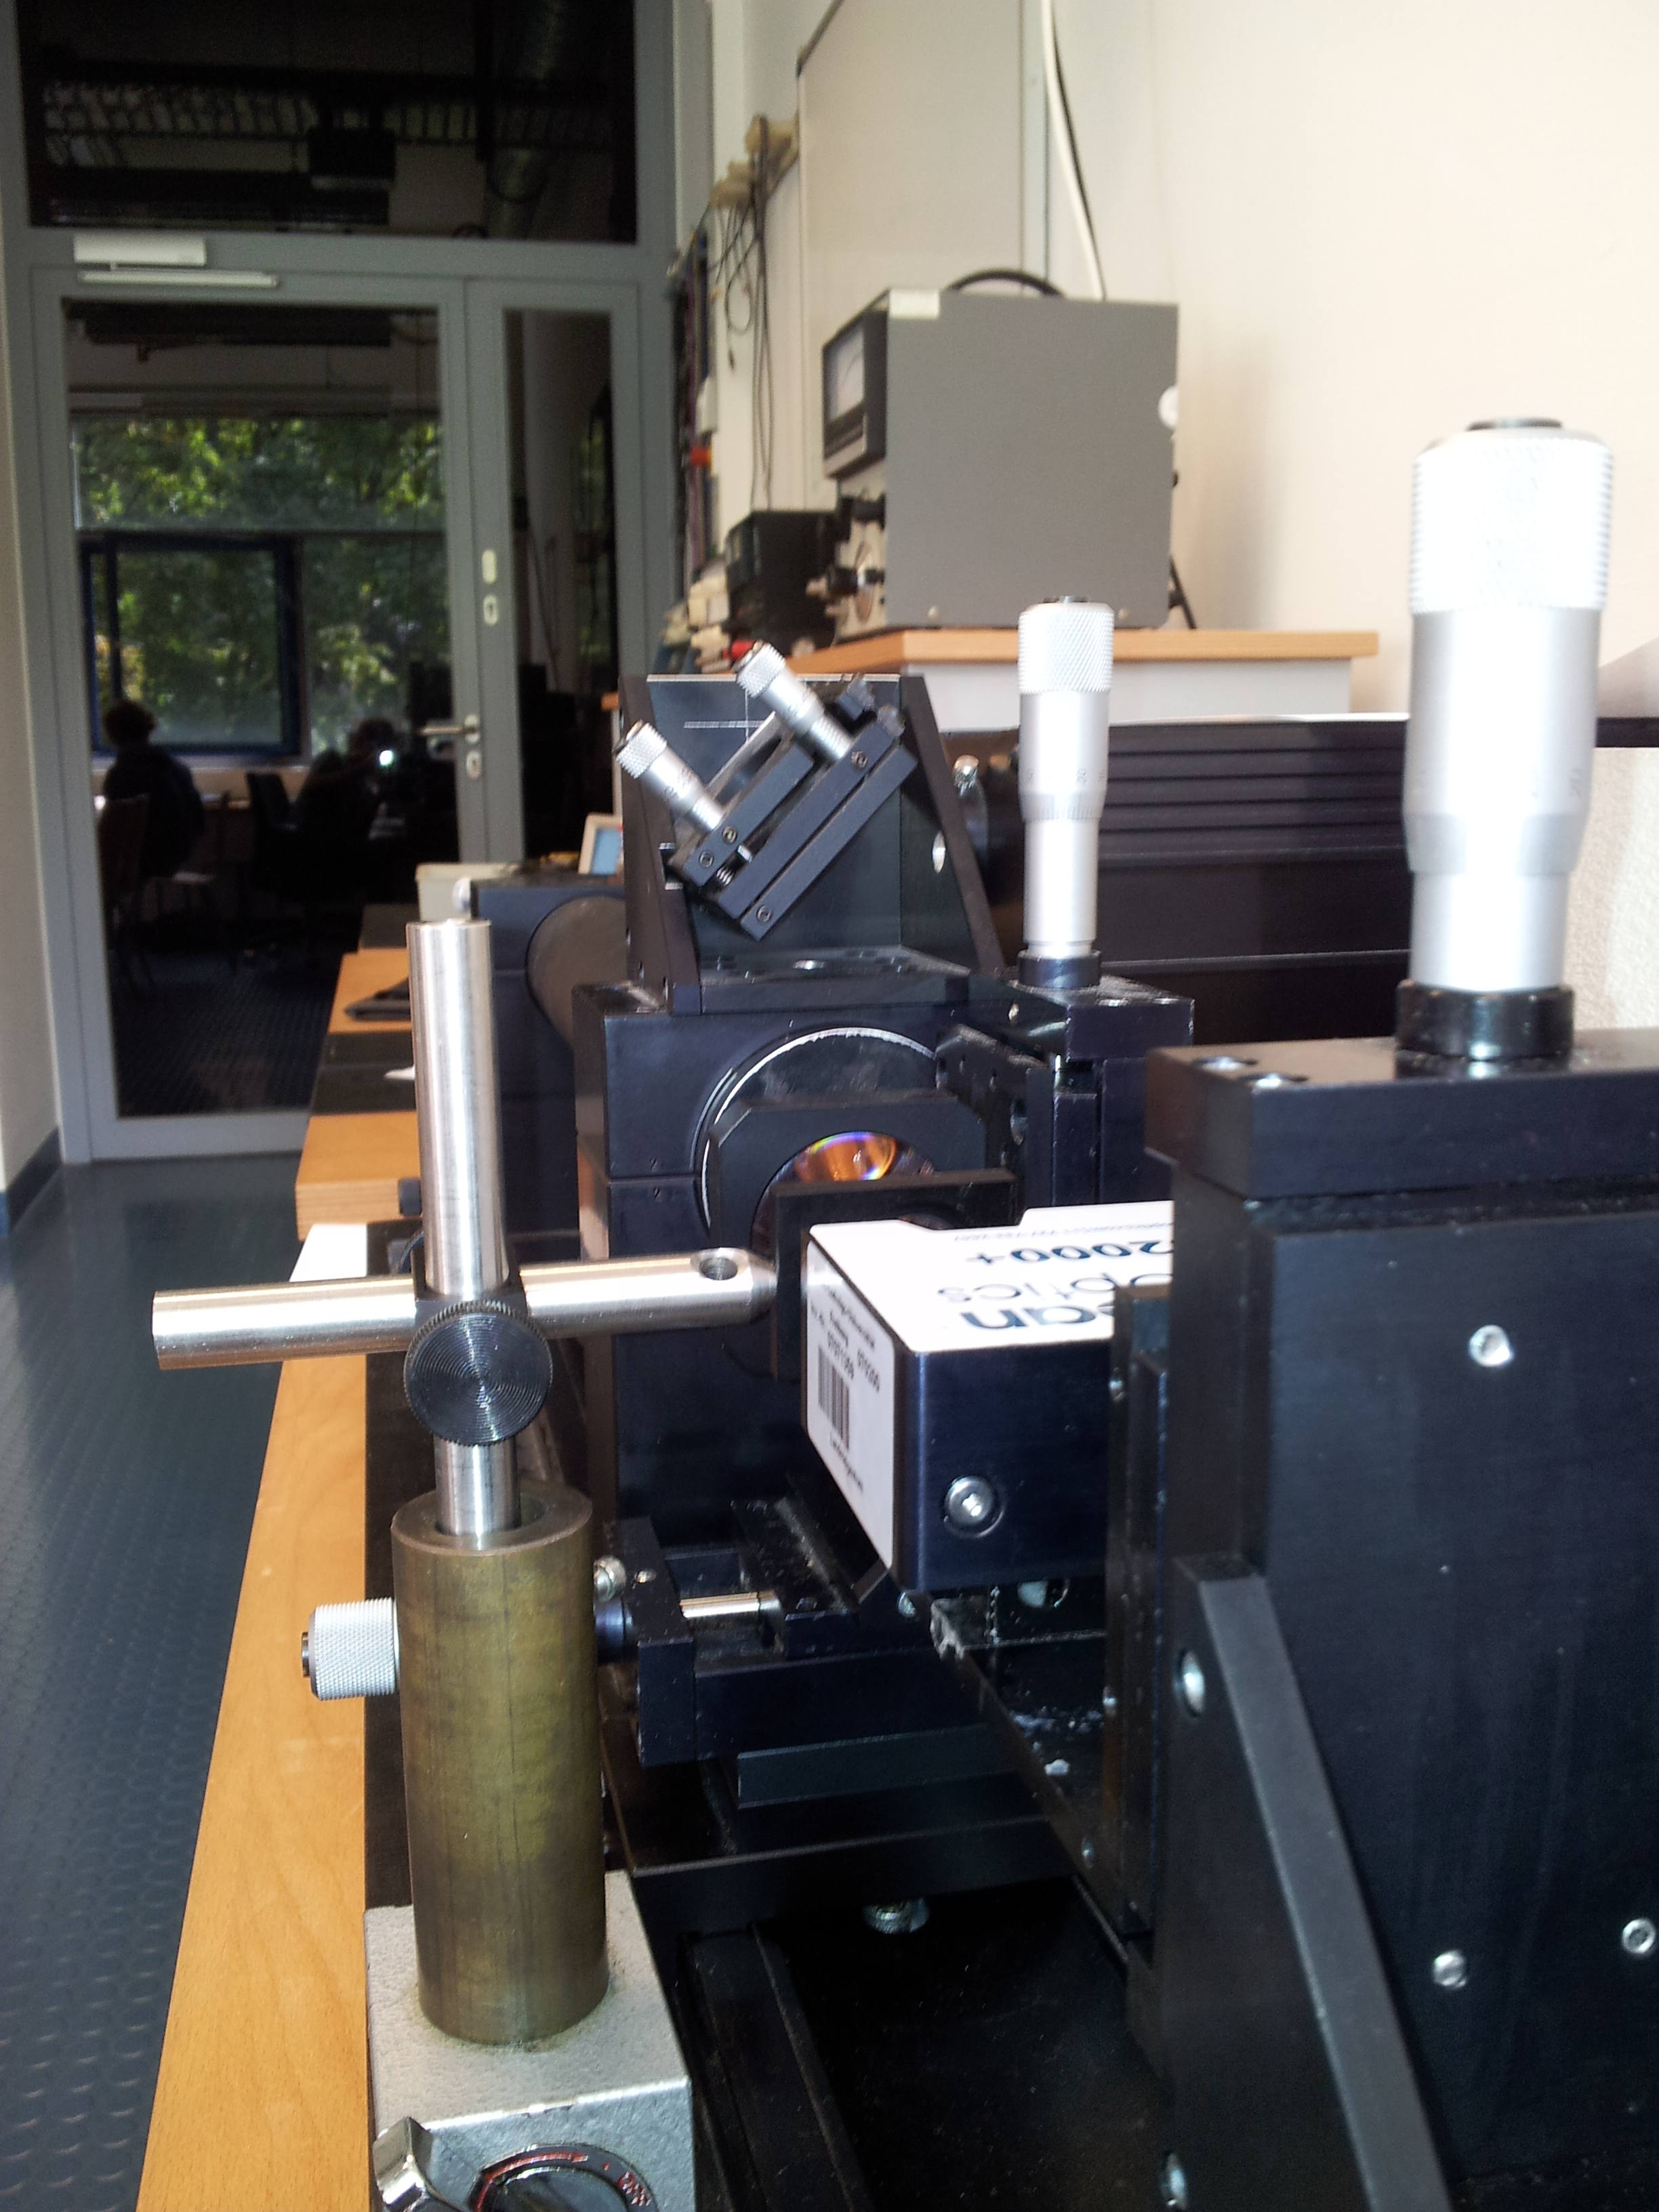
\includegraphics[width=6cm]{pics/const3}
 \label{fig:const3}
\end{SCfigure}
sample textsample textsample textsample textsample textsample text
sample textsample textsample textsample textsample textsample text
sample textsample textsample textsample textsample textsample text
sample textsample textsample textsample textsample textsample text
sample textsample textsample textsample textsample textsample text
sample textsample textsample textsample textsample textsample text
